\section{Regneregler for ubestemte integraler}
\noindent I differentialregning studerede vi problemet med at finde $f'(x)$ hvis vi kender $f(x)$. Nu vil vi i stedet betragte det inverse problem, hvordan man kan finde $f(x)$ hvis man kender $f'(x)$. For at løse dette problem vil vi introducere integralregning. 

Hvis $f$ er en kontinuert funktion, så siger vi, at $F$ er en stamfunktion til $f$, hvis der gælder at
\begin{align*}
F'(x)=f(x).
\end{align*}
Vi husker, at hvis $c \in \mathbb{R}$, så gælder der, at $\frac{d}{d x}c=0$. Det betyder, at hvis $F$ er en stamfunktion til $f$, så er 
\begin{align*}
\frac{d}{dx}(F(x)+c) = \frac{d}{dx} F(x) = f(x),
\end{align*}
også en stamfunktion til $f$. Dermed kan vi kun bestemme en stamfunktion op til en konstant (hvilket medfører at der er uendeligt mange stamfunktioner til en funktion). Vi definerer det ubestemte integral af en kontinuert funktion $f$ til at være
\begin{align*}
\int f(x) \d x = F(x) + c,
\end{align*}
hvor $c \in \mathbb{R}$ og $F$ er en stamfunktion til $f$ (se Figur~\ref{fig:ubestemtint1et}).
\begin{figure}[!htbp]
  \pgfplotsset{width=0.5\textwidth,compat=1.11}
  \centering
  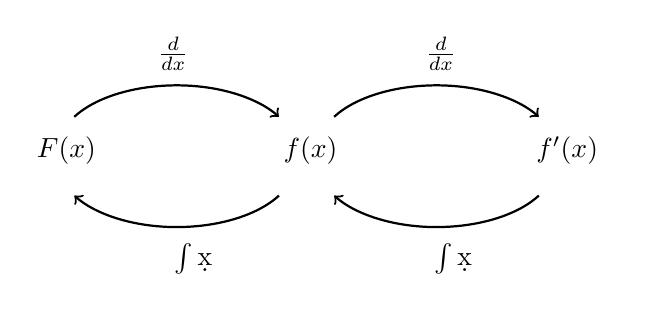
\begin{tikzpicture}
  \node[] at (3.5,1.1) [label=left:$\frac{d}{dx}$]{};
  \node[] at (6.9,1.1) [label=left:$\frac{d}{dx}$]{};
  \node[] at (3.8,-1.5) [label=left:$\int \d x$]{};
  \node[] at (7.1,-1.5) [label=left:$\int \d x$]{};
  \node[] at (1.7,0.3) [label=below:$F(x)$]{};
  \node[] at (4.8,0.3) [label=below:$f(x)$]{};
  \node[] at (8.7,0.3) [label=below left:$f'(x)$]{};
  \draw[thick,->] (1.8,0.3) arc (150:30:1.5 and 0.8);
  \draw[thick,->] (5.1,0.3) arc (150:30:1.5 and 0.8);
  \draw[thick,->] (4.4,-0.7) arc (-30:-150:1.5 and 0.8);
  \draw[thick,->] (7.7,-0.7) arc (-30:-150:1.5 and 0.8);
 \end{tikzpicture}
  \caption{Sammenhængen mellem integration og differentiation.}
  \label{fig:ubestemtint1et}
\end{figure}
\paragraph*{Eksempler:}
\begin{enumerate}
\item Vis at både $F_1(x)=x^3+2x+1$ og $F_2(x)=x^3+2x$ er stamfunktioner til $f(x)=3x^2+2$:

Vi tjekker om $F_1'(x)=f(x)$ og $F_2'(x)=f(x)$ ved at differentiere
\begin{align*}
F_1'(x)&=\frac{d}{dx}(x^3+2x+1)=3x^2+2 = f(x),\\
F_2'(x)&=\frac{d}{dx}(x^3+2x)=3x^2+2 = f(x),
\end{align*}
hvilket viser at både $F_1'$ og $F_2'$ er stamfunktioner til $f$.
\item Vis at $F(x)=e^x$ er stamfunktion til $f(x)=e^x$:

Vi tjekker om $F'(x)=f(x)$ ved at differentiere
\begin{align*}
F'(x)=\frac{d}{dx}e^x = e^x = f(x),
\end{align*}
hvilket viser at $F$ er en stamfunktion til $f$.
\end{enumerate}
\paragraph*{Regneregler:}
Hvis $f$ og $g$ begge er kontinuerte funktioner, så har vi følgende regneregler for ubestemte integraler
\begin{enumerate}
\item $\displaystyle \int c f(x) \d x = c \int f(x) \d x$, hvor $c \in \mathbb{R}$.
\item $\displaystyle \int f(x) \pm g(x) \d x = \int f(x) dx \pm \int g(x) \d x$.
\end{enumerate}
Der findes flere regneregler for ubestemte integraler, som vi vil betragte de næste par kursusgange.

\paragraph*{Tabel over funktioner og deres stamfunktioner:}
I Tabel~\ref{tab:ubestemtint1et} er der en liste, over de mest almindelige funktioner og deres stamfunktioner
\begin{table}[h!]
\centering
\begin{tabular}{l !{\qquad} {c}!}
$f(x)$      & $\int f(x) \d x$									\\ \toprule
$0$			& $c$												\\ \midrule
$k$			& $kx+c$											\\ \midrule
$x$			& $\frac{1}{2}x^2+c$								\\ \midrule
$x^n$  		& $\frac{1}{n+1} x^{n+1}+c$, $n \neq -1$			\\ \midrule
$\sqrt{x}$	& $\frac{2}{3}x^{\frac{3}{2}}+c$					\\ \midrule
$\frac{1}{x}$& $\ln \abs{x}+c$									\\ \midrule
$e^x$  		& $e^x+c$											\\ \midrule
$e^{kx}$  	& $\frac{1}{k} e^{kx}+ c$, $k \neq 0$				\\ \midrule
$\ln x$ 	& $x\ln(x)-x+c$										\\ \midrule
$a^x$  		& $\frac{1}{\ln(a)}a^x+c$, $a \neq 1$				\\ \midrule
$\log_a x$ 	& $\frac{x(\ln(x)-1)}{\ln(a)}+c$, $a \neq 1$	\\ \midrule
$\cos x$  	& $\sin x+c$										\\ \midrule
$\sin x$  	& $-\cos x+c$										\\ \midrule
$\tan x$ 	& $-\ln \vert \cos x \vert +c$						\\ \bottomrule  
\end{tabular}
\caption{Udvalgte stamfunktioner.}
\label{tab:ubestemtint1et}
\end{table}

\paragraph*{Eksempler:}
\begin{enumerate}
\item Bestem enhver stamfunktion til $f(x)=x^3+9x+1$:

Ved at benytte begge regneregler og Tabel~\ref{tab:ubestemtint1et}, får vi at
\begin{align*}
F(x) &=\int f(x) \d x  \\
&= \int (x^3+9x+1) \d x \\
&= \int x^3 \d x + 9 \int x \d x + \int 1 \d x  \\
&= \frac{1}{4}x^4 + \frac{9}{2}x^2 + x + c.
\end{align*}
\item Bestem enhver stamfunktion til $f(x)=\frac{1}{x}+\sqrt{x}+e^x$:

Ved at benytte begge regneregel $2.$ og Tabel~\ref{tab:ubestemtint1et}, får vi at
\begin{align*}
F(x) &= \int f(x) \d x  \\
&= \int \Big(\frac{1}{x}+\sqrt{x}+e^x\Big) \d x  \\
&= \int \frac{1}{x} \d x + \int \sqrt{x} \d x + \int e^x \d x  \\
&= \ln x + \frac{2}{3}x^{\frac{3}{2}} + e^x +c.
\end{align*}
\item Bestem den stamfunktion til $f(x)=3e^{3x}$, som går gennem punktet $(0,7)$:

Vi finder først enhver stamfunktion til $f$, ved at bruge regneregel $1$. og Tabel~\ref{tab:ubestemtint1et}
\begin{align*}
F(x) &= \int f(x) \d x \\
&=\int 3e^{3x} \d x  \\
&= 3 \int e^{3x} \d x  \\
&=3 \cdot \frac{1}{3} e^{3x} + c \\
&=e^{3x}+c.
\end{align*}
Da vi ved, at $F$ går gennem punktet $(0,7)$, har vi, at $F(0)=7$. Indsætter vi dette, får vi én ligning med én ubekendt som vi kan løse, for at finde $c$
\begin{align*}
F(0)=7 & \Leftrightarrow e^{3 \cdot 0} + c = 7 \\
&\Leftrightarrow 1 + c = 7 \\
&\Leftrightarrow c=6.
\end{align*}
Det giver, at den stamfunktion der går gennem punktet $(0,7)$, er $F(x)=e^{3x}+6$.
\end{enumerate}





